\subsection{Question 1}

\begin{figure}[H]
	\centering
	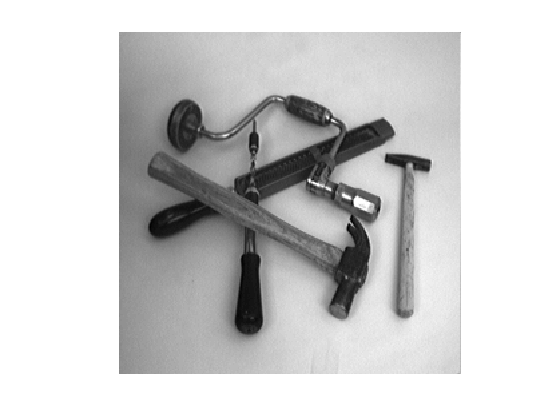
\includegraphics[scale=0.8]{./images/Q1/tools.png}
	\caption{Image \texttt{few256}.}
	\label{fig:Q1:tools}
\end{figure}


\begin{figure}[H]
	\centering
	\scalebox{0.9}{% This file was created by matlab2tikz.
%
%The latest updates can be retrieved from
%  http://www.mathworks.com/matlabcentral/fileexchange/22022-matlab2tikz-matlab2tikz
%where you can also make suggestions and rate matlab2tikz.
%
\begin{tikzpicture}

\begin{axis}[%
width=1.742in,
height=1.756in,
at={(11.472in,8.542in)},
scale only axis,
axis on top,
separate axis lines,
every outer x axis line/.append style={black},
every x tick label/.append style={font=\color{black}},
xmin=0.5,
xmax=254.5,
every outer y axis line/.append style={black},
every y tick label/.append style={font=\color{black}},
y dir=reverse,
ymin=0.5,
ymax=256.5,
hide axis,
title={SDO: X-wise derivative}
]
\addplot [forget plot] graphics [xmin=0.5,xmax=254.5,ymin=0.5,ymax=256.5] {./images/Q1/Q1-1.png};
\end{axis}

\begin{axis}[%
width=1.77in,
height=1.756in,
at={(14.852in,8.542in)},
scale only axis,
axis on top,
separate axis lines,
every outer x axis line/.append style={black},
every x tick label/.append style={font=\color{black}},
xmin=0.5,
xmax=256.5,
every outer y axis line/.append style={black},
every y tick label/.append style={font=\color{black}},
y dir=reverse,
ymin=0.5,
ymax=254.5,
hide axis,
title={SDO: Y-wise derivative}
]
\addplot [forget plot] graphics [xmin=0.5,xmax=256.5,ymin=0.5,ymax=254.5] {./images/Q1/Q1-2.png};
\end{axis}

\begin{axis}[%
width=1.742in,
height=1.756in,
at={(11.472in,6.103in)},
scale only axis,
axis on top,
separate axis lines,
every outer x axis line/.append style={black},
every x tick label/.append style={font=\color{black}},
xmin=0.5,
xmax=254.5,
every outer y axis line/.append style={black},
every y tick label/.append style={font=\color{black}},
y dir=reverse,
ymin=0.5,
ymax=256.5,
hide axis,
title={CDO: X-wise derivative}
]
\addplot [forget plot] graphics [xmin=0.5,xmax=254.5,ymin=0.5,ymax=256.5] {./images/Q1/Q1-3.png};
\end{axis}

\begin{axis}[%
width=1.77in,
height=1.756in,
at={(14.852in,6.103in)},
scale only axis,
axis on top,
separate axis lines,
every outer x axis line/.append style={black},
every x tick label/.append style={font=\color{black}},
xmin=0.5,
xmax=256.5,
every outer y axis line/.append style={black},
every y tick label/.append style={font=\color{black}},
y dir=reverse,
ymin=0.5,
ymax=254.5,
hide axis,
title={CDO: Y-wise derivative}
]
\addplot [forget plot] graphics [xmin=0.5,xmax=256.5,ymin=0.5,ymax=254.5] {./images/Q1/Q1-4.png};
\end{axis}

\begin{axis}[%
width=1.756in,
height=1.756in,
at={(11.465in,3.664in)},
scale only axis,
axis on top,
separate axis lines,
every outer x axis line/.append style={black},
every x tick label/.append style={font=\color{black}},
xmin=0.5,
xmax=255.5,
every outer y axis line/.append style={black},
every y tick label/.append style={font=\color{black}},
y dir=reverse,
ymin=0.5,
ymax=255.5,
hide axis,
title={Roberts: X-wise derivative}
]
\addplot [forget plot] graphics [xmin=0.5,xmax=255.5,ymin=0.5,ymax=255.5] {./images/Q1/Q1-5.png};
\end{axis}

\begin{axis}[%
width=1.756in,
height=1.756in,
at={(14.859in,3.664in)},
scale only axis,
axis on top,
separate axis lines,
every outer x axis line/.append style={black},
every x tick label/.append style={font=\color{black}},
xmin=0.5,
xmax=255.5,
every outer y axis line/.append style={black},
every y tick label/.append style={font=\color{black}},
y dir=reverse,
ymin=0.5,
ymax=255.5,
hide axis,
title={Roberts: Y-wise derivative}
]
\addplot [forget plot] graphics [xmin=0.5,xmax=255.5,ymin=0.5,ymax=255.5] {./images/Q1/Q1-6.png};
\end{axis}

\begin{axis}[%
width=1.756in,
height=1.756in,
at={(11.465in,1.225in)},
scale only axis,
axis on top,
separate axis lines,
every outer x axis line/.append style={black},
every x tick label/.append style={font=\color{black}},
xmin=0.5,
xmax=254.5,
every outer y axis line/.append style={black},
every y tick label/.append style={font=\color{black}},
y dir=reverse,
ymin=0.5,
ymax=254.5,
hide axis,
title={Sobel: X-wise derivative}
]
\addplot [forget plot] graphics [xmin=0.5,xmax=254.5,ymin=0.5,ymax=254.5] {./images/Q1/Q1-7.png};
\end{axis}

\begin{axis}[%
width=1.756in,
height=1.756in,
at={(14.859in,1.225in)},
scale only axis,
axis on top,
separate axis lines,
every outer x axis line/.append style={black},
every x tick label/.append style={font=\color{black}},
xmin=0.5,
xmax=254.5,
every outer y axis line/.append style={black},
every y tick label/.append style={font=\color{black}},
y dir=reverse,
ymin=0.5,
ymax=254.5,
hide axis,
title={Sobel: Y-wise derivative}
]
\addplot [forget plot] graphics [xmin=0.5,xmax=254.5,ymin=0.5,ymax=254.5] {./images/Q1/Q1-8.png};
\end{axis}
\end{tikzpicture}%}
	\caption{Derivatives of image \texttt{few256} in the $x$ and $y$ directions. The simple differences operator is featured in the first row,
	the central differences operator in the second, the Roberts cross operator in the third and the Sobel operator in the fourth.}
	\label{fig:Q1:derivatives}
\end{figure}


In the case of the simple differences operator, the kernel used has a size of $1 \times 3$ and $3 \times 1$ when considering the x-wise and y-wise 
derivatives respectively. Since \textit{all} elements of the kernel have to be multiplied by a pixel value of a $N \times M$ image (parameter \texttt{SHAPE = valid}),
the former kernel will fit exactly $N$ times into the image $x$-wise (vertically), but only $M-2$ times $y$-wise (horizontally). In the general case where
a kernel is of size $(2L+1) \times (2K+1)$, the output image's size will be $(N-L-1) \times (M-K-1)$. Table \ref{fig:Q1:kernel_sizes} shows the size of each
kernel used by each operator for taking derivatives in both $x$-wise and $y$-wise directions. Tables \ref{tbl:Q1:x_wise_sizes} and 
\ref{tbl:Q1:y_wise_sizes} illustrate the size of the output images for the various operators used to deliver edge detection.


\begin{table}
	\centering
    \begin{tabular}{c|cc}
    operator / kernel size & x\_wise   & y\_wise   \\ \hline
    SDO                    & $1 \times 3$ & $3 \times 1$ \\
    CDO                    & $1 \times 3$ & $3 \times 1$ \\
    Roberts                & $2 \times 2$ & $2 \times 2$ \\
    Sobel                  & $3 \times 3$ & $3 \times 3$ \\
    \end{tabular}
    \caption{Kernel sizes for the $4$ operators used, for taking derivatives in both $x$-wise and $y$-wise directions.}
    \label{fig:Q1:kernel_sizes}
\end{table}


\begin{table}[H]
	\centering
    \begin{tabular}{l|cc}
    image           & size\_x & size\_y \\ \hline
    few256          & $256$     & $256$     \\
    SDO(few256)     & $256$     & $254$     \\
    CDO(few256)     & $256$     & $254$     \\
    Roberts(few256) & $255$     & $255$     \\
    Sobel(few256)   & $254$     & $254$     \\
    \end{tabular}
    \caption{Image sizes for the origin image and the images of derivatives in the $x$-wise direction.}
    \label{tbl:Q1:x_wise_sizes}
\end{table}

\begin{table}[H]
	\centering
    \begin{tabular}{l|cc}
    image           & size\_x & size\_y \\ \hline
    few256          & $256$     & $256$     \\
    SDO(few256)     & $254$     & $256$     \\
    CDO(few256)     & $254$     & $256$     \\
    Roberts(few256) & $255$     & $255$     \\
    Sobel(few256)   & $254$     & $254$     \\
    \end{tabular}
    \caption{Image sizes for the origin image and the images of derivatives in the $y$-wise direction.}
	\label{tbl:Q1:y_wise_sizes}
\end{table}
